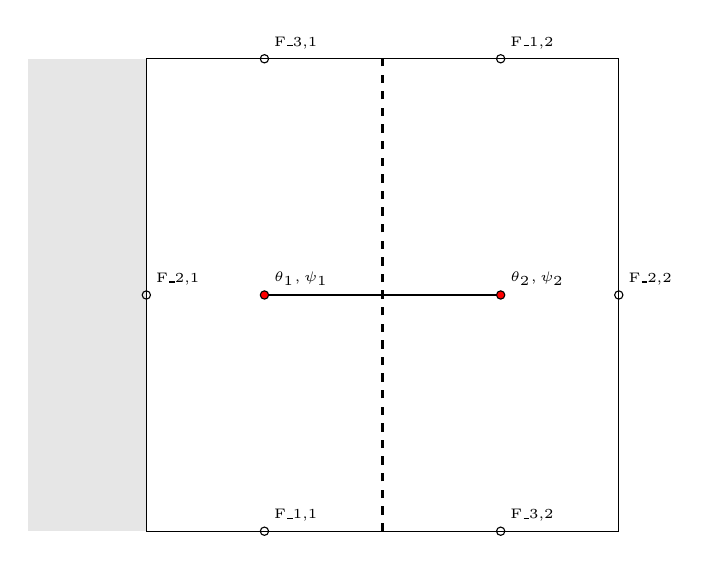
\begin{tikzpicture}

	\coordinate (P1) at (-3cm,0cm);
	\coordinate (P2) at (3cm,0cm);
	\coordinate (P3) at (3cm,6cm);
	\coordinate (P4) at (-3cm,6cm);
	\coordinate (P5) at (0cm,0cm);
	\coordinate (P6) at (0cm,6cm);

	\draw (P1) -- (P2) -- (P3) -- (P4) -- cycle;
	\draw[thick,dashed] (P5) -- (P6);

	\coordinate (P7) at (-4.5cm,0cm);
	\coordinate (P8) at (-4.5cm,6cm);	
	\coordinate (P9) at (4.5cm,6cm);
	\coordinate (P10) at (4.5cm,0cm);

	\filldraw[fill=gray] (P1) ;
	\draw -- (P7);
	[snake=zigzag] (P7) -- (P8);
	\draw  |- (P1);
	\fill[color=gray,opacity=.2] (P1) rectangle (P8) ;


	\coordinate (F11) at (-1.5cm,0cm);
	\coordinate (F21) at (-3cm,3cm);
	\coordinate (F31) at (-1.5cm,6cm);
	\coordinate (F12) at (1.5cm,6cm);
	\coordinate (F22) at (3cm,3cm);
	\coordinate (F32) at (1.5cm,0cm);	

	\coordinate (N1) at (-1.5cm,3cm);
	\coordinate (N2) at (1.5cm,3cm);

	\draw[thick] (N1) -- (N2);

	\foreach \i in {1,2,3}
	{
	  \draw[] (F\i1) circle (0.15em)
	    node[above right] {\tiny F\_{\i,1}};
	}
	\foreach \i in {1,2,3}
	{
	  \draw[] (F\i2) circle (0.15em)
	    node[above right] {\tiny F\_{\i,2}};
	}



	\draw[fill=red] (N1) circle (0.15em)
	    node[above right] {\tiny $\theta_{1},\psi_{1}$};
	\draw[fill=red] (N2) circle (0.15em)
	    node[above right] {\tiny $\theta_{2},\psi_{2}$};
\end{tikzpicture}



